\documentclass{report}

\usepackage{geometry}
\geometry{a4paper,total={170mm,257mm},left=20mm,top=20mm}
\usepackage[utf8]{inputenc}
\usepackage{amsmath}
\usepackage{amsfonts}
\usepackage{amsthm}
\usepackage{amssymb}
\usepackage{bm}
\usepackage{graphicx}
\usepackage{paralist}
\usepackage[dvipsnames]{xcolor}
\usepackage{caption}
\usepackage{subcaption}
\usepackage{hyperref}
\hypersetup{urlbordercolor=ForestGreen,linkbordercolor=RoyalPurple}
\usepackage{tikz}
\usetikzlibrary{positioning}
\usetikzlibrary{intersections}
\usepackage{algpseudocode}
\usepackage{algorithm}
\usepackage{titling}
\usepackage{pgfplots}
\usepackage{fontawesome5}

%%% Tento soubor obsahuje definice různých užitečných maker a prostředí %%%
%%% Další makra připisujte sem, ať nepřekáží v ostatních souborech.     %%%

%%% Drobné úpravy stylu

% Tato makra přesvědčují mírně ošklivým trikem LaTeX, aby hlavičky kapitol
% sázel příčetněji a nevynechával nad nimi spoustu místa. Směle ignorujte.
\makeatletter
\def\@makechapterhead#1{
  {\parindent \z@ \raggedright \normalfont
   \Huge\bfseries \thechapter. #1
   \par\nobreak
   \vskip 20\p@
}}
\def\@makeschapterhead#1{
  {\parindent \z@ \raggedright \normalfont
   \Huge\bfseries #1
   \par\nobreak
   \vskip 20\p@
}}
\makeatother

% Toto makro definuje kapitolu, která není očíslovaná, ale je uvedena v obsahu.
\def\chapwithtoc#1{
\chapter*{#1}
\addcontentsline{toc}{chapter}{#1}
}

% Trochu volnější nastavení dělení slov, než je default.
\lefthyphenmin=2
\righthyphenmin=2

% Zapne černé "slimáky" na koncích řádků, které přetekly, abychom si
% jich lépe všimli.
\overfullrule=1mm

%%% Makra pro definice, věty, tvrzení, příklady, ... (vyžaduje baliček amsthm)

\theoremstyle{plain}
\newtheorem{veta}{Věta}
\newtheorem{lemma}[veta]{Lemma}
\newtheorem{tvrz}[veta]{Tvrzení}

\theoremstyle{plain}
\newtheorem{definice}{Definice}
\newtheorem*{pozor}{Pozorování}
\newtheorem*{cvic}{Cvičení}
\newtheorem*{fakt}{Fakt}

\theoremstyle{remark}
\newtheorem*{dusl}{Důsledek}
\newtheorem*{pozn}{Poznámka}
\newtheorem*{prikl}{Příklad}

\theoremstyle{plain}
\newtheorem{thm}{Theorem}
%\newtheorem{lemma}[thm]{Lemma}
\newtheorem{claim}[thm]{Claim}

\theoremstyle{plain}
\newtheorem{defn}{Definition}
\newtheorem*{observ}{Observation}
\newtheorem*{exerc}{Exercise}
\newtheorem*{fact}{Fact}

\theoremstyle{remark}
\newtheorem*{cor}{Corollary}
\newtheorem*{rem}{Remark}
\newtheorem*{example}{Example}


%%% Prostředí pro důkazy

\newenvironment{dukaz}{
  \par\medskip\noindent
  \textit{Důkaz}.
}{
\newline
\rightline{$\qedsymbol$}
}

\newenvironment{myproof}{
	\par\medskip\noindent
	\textit{Proof}.
}{
	\newline
	\rightline{$\qedsymbol$}
}


%%% Prostředí pro sazbu kódu, případně vstupu/výstupu počítačových
%%% programů. (Vyžaduje balíček fancyvrb -- fancy verbatim.)

\DefineVerbatimEnvironment{code}{Verbatim}{fontsize=\small, frame=single}

%%% Prostor reálných, resp. přirozených čísel
\newcommand{\R}{\mathbb{R}}
\newcommand{\N}{\mathbb{N}}
\newcommand{\Z}{\mathbb{Z}}

%%% Užitečné operátory pro statistiku a pravděpodobnost
\DeclareMathOperator{\pr}{\textsf{P}}
\DeclareMathOperator{\E}{\textsf{E}\,}
\DeclareMathOperator{\var}{\textrm{var}}
\DeclareMathOperator{\sd}{\textrm{sd}}

%%% Příkaz pro transpozici vektoru/matice
\newcommand{\T}[1]{#1^\top}

%%% Vychytávky pro matematiku
\newcommand{\goto}{\rightarrow}
\newcommand{\gotop}{\stackrel{P}{\longrightarrow}}
\newcommand{\maon}[1]{o(n^{#1})}
\newcommand{\abs}[1]{\left|{#1}\right|}
\newcommand{\dint}{\int_0^\tau\!\!\int_0^\tau}
\newcommand{\isqr}[1]{\frac{1}{\sqrt{#1}}}

%%% Vychytávky pro tabulky
\newcommand{\pulrad}[1]{\raisebox{1.5ex}[0pt]{#1}}
\newcommand{\mc}[1]{\multicolumn{1}{c}{#1}}


% set up \maketitle to accept a new item
\predate{\begin{center}\placetitlepicture\large}
	\postdate{\par\end{center}}

% commands for including the picture
\newcommand{\titlepicture}[2][]{%
	\renewcommand\placetitlepicture{%
		\includegraphics[#1]{#2}\par\medskip
	}%
}
\newcommand{\placetitlepicture}{} % initialization


\usepackage{babel}

% For Matroids.
\newcommand{\M}{\mathcal{M}}
\newcommand{\I}{\mathcal{I}}
\newcommand{\C}{\mathcal{C}}
\newcommand{\B}{\mathcal{B}}
\DeclareMathOperator{\rank}{\textsf{r}}
\newcommand{\dual}[1]{#1^{\ast}}

%%% DOCUMENT
\title{Matroid Theory}
\author{Tomáš Turek\thanks{These are my notes on the course Matroid Theory, which was taught by Ondřej Pangrác in the year 2024. \INFO}}
\titlepicture[width=3in]{res/vamos.pdf}
\date{\today}

\begin{document}
	\maketitle
	\tableofcontents
	\chapter{Basic definitions}

\begin{defn}
	\textbf{Matroid} $\M = (E, \I)$ is for $E$ finite non-empty set and $\I \subseteq 2^E$ (also called as independent sets) satisfying these properties:
	
	\begin{enumerate}[(\text{I}1)]
		\item $\emptyset \in \I$,
		\item $I \in \I \Rightarrow \forall I' \subseteq I : I' \in \I$,
		\item $I_1, I_2 \in \I, \abs{I_1} < \abs{I_2} \Rightarrow \exists e \in I_2 \setminus I_1: I_1 \cup \{e\} \in \I$.
	\end{enumerate}
\end{defn}

\begin{notation}
	For further use and simplification we will sometimes use $I + e$ as a substitution for $I \cup \{e\}$. Similarly also $I - e$ for $I \setminus \{e\}$.
\end{notation}

\begin{example}
	For a given multi-graph $G = (V,F)$ we will set $E = F$ (or in other words $E$ stands for edges and the set). Independent sets $\I$ will be all acyclic subsets of $E$. Easily seen (I1) and (I2) is satisfied. For the third one (I3) it is also quite easily seen, because if we have one larger and smaller non-cycles then we can append one edge from the larger to the smaller.
\end{example}

\begin{example}
	Let $E$ be some elements of a vector space $V$. If $X \subseteq E$ is independent then it is linearly independent in $V$.
\end{example}

\begin{defn}
	Matroid \textbf{isomorphism} for two matroids $\M_i = (E_i, \I_i)$ for $i = 1,2$ is a bijection $f: E_1 \to E_2$ satisfying $\forall X \subseteq E_i : X \in \I_1 \Leftrightarrow f(X) \in \I_2$.
\end{defn}

\section{Circuits}

\begin{defn}
	$X \subseteq E$ is a \textbf{circuit} if $X \notin \I$ and $\forall x \in X : X - x \in \I$. Also we will denote $\C(\M)$ as the set of all circuits of $\M$.
\end{defn}

\begin{lemma}
	Let $\M = (E, \I)$ be a matroid and $\C$ its collection of circuits, then
	
	\begin{enumerate}[(C1)]
		\item $\emptyset \notin \C$,
		\item $\forall C_1, C_2 \in \C : C_1 \subseteq C_2 \Rightarrow C_1 = C_2$ and
		\item $C_1, C_2 \in \C, C_1 \neq C_2, e \in C_1 \cap C_2 \Rightarrow C_3 \subseteq (C_1 \cup C_2) -e , C_e \in \C$.
	\end{enumerate}
\end{lemma}

\begin{proof}
	(C1) and (C2) are easily seen from (I1) and (I2). Now for the third part (C3). So for contradiction let $C_1, C_2, e$ be as mentioned in the first part, but $(C_1 \cup C_2) - e \in \I$. Then $\exists f \in C_2 \setminus C_1 : C_2 - f \in \I$. Now find $I \in \I$ max s.t. $C_2 \setminus \{f\} \subseteq I \subseteq C_1 \cup C_2$. If $f \notin I$ then it would contain $C_2$ which is dependent and $\exists g \in C_1 \setminus C_2 : g \notin I$ otherwise it would contain $C_1$ which is dependent. Therefore
	
	$$
	|I| \leq | C_1 \cup C_2 | - 2 < |(C_1 \cup C_2) - e|
	$$
	
	\noindent and now we may use the third axiom (I3) that is $\exists x \in |(C_1 \cup C_2) - e| \setminus I$ s.t. $I + e \in \I$ (this cannot be otherwise $I$ contains the whole $C_2$). Now $I + x$ contradicts the maximality of $I$.
\end{proof}

\begin{claim}
	Lets have $E$ and $\C \subseteq 2^E$ satisfying all (C1), (C2) and (C3). Then set $\I = \{X \subseteq E | \forall C \in \C : C \nsubseteq X\}$ and $\M = (E, \I)$ is a matroid.
\end{claim}

\begin{proof}
	We have to show all properties of matroid. That is (I1) is trivially satisfied and (I2) also trivially holds. For the last (I3) we use a contradiction. For that we have $I_1, I_2 \in \I$, then $\forall e \in I_2 \setminus I_1 : I_1 + e \notin \I$. Let $I_3 \subseteq I_1 \cup I_2$ s.t. $|I_3| > |I_1|$ and $|I_1 \setminus I_3|$ is minimal. If $|I_1 \setminus I_3|$ would be empty then (I3) will hold, therefore assume it is non-empty.
	
	Fix $e \in I_1 \setminus I_3$. Let $I_k = |I_3 - f| +e$ for $(f \in I_3 \setminus I_1)$. This cannot be independent ($\notin \I$) therefore $\exists C_k \subseteq T_k : C_k \in \C$ and $f \notin C_k, e \in C_k$.
	
	$(I_3 \setminus I_1) \cap C_k = \emptyset$ hence $C_k \subseteq T_k \setminus (I_3 \setminus I_1) = (I_1 \cap I_3) + e \subseteq I_1$ this is not possible so it must be non-empty. Then $\exists g \in (I_3 \setminus I_1) \cap C_k \Rightarrow C_k, C_g \in \C, e \in C_k \cap C_g, f \notin C_k, g \notin C_g$ but $(C_k \cup C_g) - e \subseteq I_3$ which is contradiction with (C3).
\end{proof}

\section{Basis}

\begin{defn}
	Let $\M = (E, \I)$ be a matroid. Then $B$ is a \textbf{basis} iff $B \in \I, \forall x \in E \setminus B: B + x \notin \I$.
\end{defn}

\begin{prop}
	Let $B_1, B_2$ be bases of $\M$, then $\abs{B_1} = \abs{B_2}$.
\end{prop}

\begin{proof}
	If $|B_1| < |B_2|$ then by (I3) $\exists x \in B_2 \setminus B_1 : B_1 + x \in \I$.
\end{proof}

\begin{defn}
	Let $\B (\M) = \{B \subseteq E , B \text{ is a basis}\}$ be a collection of basis satisfying
	
	\begin{enumerate}[(B1)]
		\item $\B \neq \emptyset$ and
		\item $B_1, B_2 \in \B, e \in B_1 \setminus B_2 \Rightarrow \exists f \in B_2 \setminus B_1 : |B_1 - e| + f \in \B$.
	\end{enumerate}
\end{defn}

One can see that (B2) can be proven using $I_1 - e =: B_1$ and $I_2 = B_2$.

\begin{prop}
	Let $E \neq \emptyset$ finite set and $\B \subseteq 2^E$ satisfying (B1) and (B2). Let $\I = \{X \subseteq E : \exists B \in \B\ : X \subseteq B\}$ then $\M = (E, \I)$ is a matroid.
\end{prop}

\begin{proof}
	(I1) and (I2) are trivial. For (I3) use the following lemma.
	
	\begin{lemma}
		Let $\B$ be such that it satisfies (B1) and (B2). Then $\forall B_1, B_2 \in \B : |B_1| = |B_2|$.
	\end{lemma}
	
	\begin{proof}
		By contradiction suppose $\abs{B_1} > \abs{B_2}$ with minimal $\abs{B_1 \setminus B_2}$. Then $e \in B_1 \setminus B_2 \Rightarrow \exists f \in B_2 \setminus B_1: (B_1 - e) + f \in \B$ and also $\abs{(B_1 - e) + f} = |B_1|$ which leads to $\abs{((B_1 - e) + f) \setminus B_2} < \abs{B_1 \setminus B_2}$ which is a contradiction with the minimality.
	\end{proof}
\end{proof}

\section{Rank function}

\begin{defn}
	For a matroid $\M = (E, \I)$ define a \textbf{rank function} $\rank : 2^E \to \Z^+_0$, such that $\rank(X) = \max_{I \subseteq X, I \in \I} |I|$ and $\rank (\M) = \rank(E)$.
\end{defn}

\begin{claim}
	Rank function has the following properties:
	
	\begin{enumerate}[(R1)]
		\item $X \subseteq E: 0 \leq \rank (X) \leq |X|$,
		\item $X \subseteq Y \subseteq E \Rightarrow \rank (X) \leq \rank(Y)$ and
		\item $X, Y \subseteq E : \rank(X \cup Y) + \rank(X \cap Y) \leq \rank(X) + \rank(Y)$ (which is called \textbf{submodularity}).
	\end{enumerate}
\end{claim}

\begin{proof}[Proof of the properties]
	While (R1) and (R2) are obvious and now we will show that (R3) also holds. Let $I_1$ be the max independent in $X \cap Y$ and $I_2$ be an extension $I_2 \supseteq I_1$ and max independent in $X \cup Y$. Now $\rank(X \cup Y) + \rank(X \cap Y) = \abs{I_2} + \abs{I_1}$ and also $|I_2 \cap X| \leq \rank(X)$ and $|I_2 \cap Y| \leq \rank(Y)$. We apply simple rule $|A| + |B| = |A \cup B| + |A \cap B|$ and get
	
	$$
	\rank(X) + \rank(Y) \geq |I_2 \cap X| + |I_2 \cap Y| = |I_2| + |I_1| = \rank(X \cup Y) + \rank(X \cap Y)
	$$
\end{proof}

\begin{thm}
	For $E \neq \emptyset$ finite set and $\rank: 2^E \to \Z^+_0$ satisfying (R1), (R2) and (R3). Then $\I = \{X \subseteq E | \rank(X) = |X| \}$ and $\M = (E, \I)$ is a matroid.
	\label{rank-func-thm}
\end{thm}

\begin{lemma}
	For $E \neq \emptyset$ finite set and $\rank: 2^E \to \Z^+_0$ satisfying (R1), (R2) and (R3). It holds that if $X, Y \subseteq E$ $\forall y \in Y: \rank(X) = \rank(X + y)$ then $\rank(X) = \rank(X \cup Y)$.
	\label{rank-func-lemma}
\end{lemma}

\begin{proof}[Proof of lemma \ref{rank-func-lemma}]
	Let $Y \setminus X = \{y_1, y_2, \dots, y_k\}$ and now we will prove it by induction on $k$. For $k = 1$ it obviously holds. For $k \geq 2$ we use the submodularity.
	
	$$
	\begin{aligned}
		&\rank(X) + \rank(X) &= &\rank(X \cup \{y_1, y_2, \dots, y_{k-1}\}) + \rank(X + y_k) &\geq \rank(X \cup \{y_1, y_2, \dots, y_k\}) + \rank(X)\\
		&                    &  & \text{\small{(by induction hypothesis)}}\\
		&\rank(X)            &= &                                                            &\geq \rank(X \cup \{y_1, y_2, \dots, y_k\})\\
		&\rank(X)            &  &                                                            &\geq \rank(X \cup Y)\\
	\end{aligned}
	$$
	
	\noindent For the other inequality we use (R2) and hence we obtain equality.
\end{proof}

\begin{proof}[Proof of theorem \ref{rank-func-thm}]
	\TODO{Finish the proof.}
\end{proof}

\TODO{Insert missing part.}

\section{Uniform matroids}

\begin{defn}
	For $0 \leq r \leq n \neq 0, |E| = n$ and $\I = \{X \subseteq E : |X| \leq r\}$ is \textbf{Uniform matroid} $U_{r,n} = (E, \I)$.
\end{defn}

All the properties should be formally proven, but one can already see that all (I1), (I2) and (I3) are really satisfied. Now we will show us some examples.

\TODO{Add examples.}

\section{Visualization of matroids}

\TODO{Finish this part.}

\section{(Direct) Sum of matroids (also disjoint union)}

\begin{defn}
	We have two matroids $\M_i = (E_i, \I_i)$ for $i= 1,2$, then the (direct) sum $\M_1 \bigoplus \M_2$ is defined as a matroid $\M = (E, \I)$ where $E = E_1 \dot\cup E_2$ and $\I = \{X \subseteq E, X \cap E_i \in \I_i, i=1,2\}$.
\end{defn}

\begin{observ}
	Lets see the basis and circuits:
	
	$$
	\begin{aligned}
		&\B(\M_1 \bigoplus \M_2) = \{B_1 \cup B_2, B_i \in \B_i, i = 1,2\}\\
		&\C(\M_1 \bigoplus \M_2) = \C_1 \cup \C_2\\
		&X \subseteq E : \rank(X) = \rank_1(X \cap E_1) + \rank_2(X \cap E_2)
	\end{aligned}
	$$
\end{observ}
	\chapter{Duals \& Minors}

\section{Duals}

Firstly we will take a look at duals of matroids.

\begin{claim}
	Let $\M = (E, \I)$ be a matroid and $\B$ its bases. We set $\dual{\B} = \{E \setminus B : B \in \B\}$ then $\dual{\B}$ satisfies (B1) and (B2).
\end{claim}

\begin{proof}
	Firstly (B1) is easy. For (B2) $(E \setminus B_1), (E \setminus B_2) \in \dual{\B}, \forall e \in (E \setminus B_1) \setminus (E \setminus B_2) = B_2 \setminus B_1, \exists f \in B_1 \setminus B_2 = (E \setminus B_2) \setminus (E \setminus B_1)$. Now we apply (B2') and get that $(B_1 - f) + e \in \B$ then $E \setminus ((B_1 -f) +e) =((E \setminus B_1) -e ) + f$.
\end{proof}

Therefore $\exists \dual{\M}$ matroid with $\B(\dual{\M}) = \dual{\B}$ which will be called a \textbf{dual}. Generally we will denote duals $\M$ as $\dual{\M}$. Also we will call such elements with a prefix co-. For example $\dual{\B}$ will be a co-bases and so on.

\begin{observ}
	$\dual{(\dual{\M})} = \M$
\end{observ}

\begin{prop}
	There are two basic observations:
	
	\begin{enumerate}
		\item $\rank(\M) + \rank(\dual{\M}) = |E|$
		\item $\forall X \subseteq E : \dual{\rank}(X) = |X| - \rank(\M) + \rank(E \setminus X)$
	\end{enumerate}
	\label{rank-prop}
\end{prop}

\begin{proof}
	1. is obvious from the definitions. 2. we denote $\dual{I}$ as the max independent subset of $X$ in $\dual{\M}$ and $I$ as the max independent subset of $E \setminus X$ in $\M$. Then $\exists B \in \B, B \cap \dual{I} = \emptyset$. We may assume $I \subseteq B \Rightarrow \rank(B) = |B| = \rank(\M)$.
	
	$$
	\begin{aligned}
		B &\subseteq E \setminus \dual{I}\\
		\rank(B) &\leq \rank(E \setminus \dual{I}) \leq \rank(\M) \text{ therefore we get equality}\\
		\rank(B) &= \rank(E \setminus \dual{I})
	\end{aligned}
	$$
	
	\noindent Let $\dual{B} = E \setminus B$ be the basis of $\dual{\M}$ and $\dual{I} \subseteq \dual{B}$, moreover $\dual{I} = \dual{B} \cap X$. Also $I = B \cap (E \setminus X)$.
	
	$$
	|X| = |X \cap B| + |X \cap \dual{B}| = |B| - |I| + |\dual{I}| = \rank(\M) - \rank(E \setminus X) + \dual{\rank}(X)
	$$
\end{proof}

\begin{defn}
	We say that $H \subseteq E$ is a \textbf{hyperplane} in $\M$ if $H$ is $\subseteq$-max subset with $\rank(H) < \rank(\M)$. Or in other words
	
	$$
	\forall e \in E \setminus H : \rank(H) < \rank(H+e) < \rank(\M) \text{ so } \rank(H) = \rank(\M)-1
	$$
\end{defn}

\begin{lemma}
	For a matroid $\M = (E, \I)$ the following holds:
	
	$$
	\forall \dual{C} \subseteq E, \dual{C} \in \dual{\C}(\M) \Leftrightarrow E \setminus \dual{C} \text{ is a hyperplane of } \M.
	$$
\end{lemma}

\begin{proof}
	"$\Rightarrow$" Suppose $\dual{C} \in \dual{\C}$ by the dual of proposition \ref{rank-prop} we get
	
	$$
	\begin{aligned}
		\rank(X) &= |X| - \dual{\rank}(\M) + \dual{\rank}(E \setminus X)\\
		\rank(E \setminus \dual{C}) &= |E \setminus \dual{C}| - \dual{\rank}(\M) + \dual{\rank}(\dual{\C})\\
		&= |E| - |\dual{C}| - \dual{\rank}(\M) + |\dual{C}| - 1\\
		&= \rank(\M) - 1
	\end{aligned}
	$$
	
	\noindent then this is maximal with this property, therefore it is a hyperplane.
	
	"$\Leftarrow$" is analogous.
\end{proof}

Lets now diverge to the graphic matroids, where when we decrease $\rank(\M)$ by 1 this will result in increasing components of connectivity; hence co-circuits are edge-cuts.

\begin{prop}
	Let $\M = (E, \I)$ be a matroid, $C \in \C, \dual{C} \in \dual{\C}$ then $|C \cap \dual{C}| \neq 1$.
\end{prop}

\begin{proof}
	By contradiction assume that $C \cap \dual{C} = \{e\}$. Lets define $H = E \setminus \dual{C}$ a hyperplane for which $e \notin H$. Now we compute the following
	
	$$
	\begin{aligned}
		\rank(C) + \rank(E) &= \rank(C - e) + \rank(H + e) \\
		&= \rank(C \cap H) + \rank(C \cup H) \\
		&\leq \rank(C) + \rank(H) \\
		&= \rank(H) + \rank(E) - 1 \text{, which is a contradiction.}
	\end{aligned}
	$$
\end{proof}

Now we take a look at how does a direct sum of duals look like.

$$
\begin{aligned}
	\B(\dual{(\M_1 \bigoplus \M_2)}) &= \{E \setminus B, B \in \B(\M_1 \bigoplus \M_2)\}\\
	&= \{E \setminus (B_1 \cup B_2), B_1 \in \B_1, B_2 \in \B_2\}\\
	&= \{(E_1 \cup E_2) \setminus (B_1 \cup B_2), B_1 \in \B_1, B_2 \in \B_2\}\\
	&= \{(E_1 \setminus B_1) \cup (E_2 \setminus B_2), B_1 \in \B_1, B_2 \in \B_2\}\\
	&= \{\dual{B_1} \cup \dual{B_2}, \dual{B_1} \in \dual{\B}(\M_1), \dual{B_2} \in \dual{\B}(\M_2)\}\\
	&= \B (\dual{\M_1} \bigoplus \dual{\M_2})
\end{aligned}
$$

\noindent Therefore we may say that $\dual{(\M_1 \bigoplus \M_2)} = \dual{\M_1} \bigoplus \dual{\M_2}$.

\section{Minors}

Reader may already know minors in graph theory. They are made by two operations. Deletions of vertices and edges and contractions of edges. For minors it will work similarly, therefore we define such operations.

\begin{defn}[Deletion]
	For a matroid $\M = (E, \I)$ for $T \subseteq E$ we define $\M \setminus T = (E \setminus T, \I')$ where $\I' = \{I \in \I, I \subseteq E \setminus T\}$.
\end{defn}

\begin{defn}[Contraction]
	$\M / T = \dual{(\dual{\M} \setminus T)}$
\end{defn}

\begin{prop}
	For $\M = (E, \I), T \subseteq E$ assume $X \subseteq E \setminus T$, then
	
	\begin{enumerate}
		\item $\rank_{\M \setminus T} (X) = \rank_{\M} (X)$ and
		\item $\rank_{\M / T}(X) = \rank_{\M}(X \cup T) - \rank_{\M}(T)$.
	\end{enumerate}
\end{prop}

\begin{proof}
	1. can be easily seen. For 2. we de the following computation.
	
	$$
	\begin{aligned}
		\rank_{\M / T} (X) &= \dual{\rank_{\dual{\M} \setminus T}} (X) \\
		&= |X| - \rank_{\dual{\M} \setminus T} (E \setminus T) + \rank_{\dual{\M} \setminus T} ((E \setminus T) \setminus X)\\
		&= |X| - \dual{\rank}(E \setminus T) + \dual{\rank}(E \setminus (T \cup X)) \\
		&= |X| - (|E \setminus T| - \rank(E) + \rank(T)) + |E \setminus (T \cup X)| - \rank(E) + \rank(E \setminus (E \setminus (T \cup X))) \\
		&= |X| - |E| + |T| + |E| - |T| - |X| + \rank(E) - \rank(E) - \rank(T) + \rank(T \cup X)\\
		&=\rank(T \cup X) - \rank(T)
	\end{aligned}
	$$
\end{proof}

\begin{prop}
	We can prove that $\M ? T = (E \setminus T, \I')$ where $\I' = \{I \subseteq E \setminus T | I \cup B_T \in \I\}$, where $B_T$ is max independent subset of $T$.
\end{prop}

\begin{proof}
	In one direction lets have $I \subseteq E \setminus T$ s.t. $U \cup B_T \in \I$ now its rank has to be equal to its size.
	
	$$
	\begin{aligned}
		\rank_{\M / T} (I) &= \rank (I \cup T) - \rank(T)\\
		&= \rank(I \cup B_T) - \rank(B_T)\\
		&=|I \cup B_T| - |B_T|\\
		&= |I| + |B_T| - |B_T| = |I|
	\end{aligned}
	$$
	
	Now the other direction. For that lets have $X \in \I'$ then the following holds.
	
	$$
	\begin{aligned}
		|X| &= \rank_{\M / T}(X) = \rank(X \cup T) - \rank(T) = \rank(X \cup T) - \rank(B_T) = \rank(X \cup B_T) - |B_T|\\
		|X \cup B_T| &= |X| + |B_T| = \rank(X \cup B_T) \Rightarrow X \cup B_T \in \I
	\end{aligned}
	$$
\end{proof}

Therefore we may say that for dual it is true that: $B' \in \B(\M /T) \Leftrightarrow \exists B_T \in \B(\M | T)$ s.t. $B' \cup B_T \in \B(\M)$ where existential kvantificator can be replaced by for all. Also on notation $\M | T =  \M \setminus (E \setminus T)$ called the \textit{restriction}.

\begin{prop}
	$\C (\M /T)$ are minimal non-empty members $\{C \setminus T| C \in \C(\M)\}$.
\end{prop}

\begin{proof}
	For "$\Rightarrow$" consider $C_1 \in \C(\M / T)$ and $B_T$ max independent in $\M | T$. $C_1 \cup B_T \notin \I, \forall e \in C_1 : (C_1 - e) \cup B_T \in \I$ and therefore $\exists C \in \C(\M)$ s.t. $C_1 \subseteq C \subseteq C_1 \cup B_T \Rightarrow C_1 = C \setminus B_T = C \setminus T$.
	
	Now for "$\Leftarrow$" let $D \setminus T$ be min non-empty member $\{C \setminus T | C \in \C(\M)\}$ so $D \cap T \subsetneq D \Rightarrow D \cap T \in \I \Rightarrow \exists B_T$ max independent in $\M |T$ s.t. $D \cap T \subseteq B_T$ and now $D \subseteq D \cup B_T = (D \setminus T) \cup B_T \notin \I$ because it contains a circuit $\Rightarrow (D \setminus T) \notin \I(\M / T)$ therefore $\exists D' \in \C (\M / T) : D' \subseteq D \setminus T$ if $D' \subsetneq D \setminus T$ then it would contradicts the minimality.
\end{proof}

\begin{claim}
	For $\M = (E, \I), T_1, T_2 \subseteq E, T_1 \cap T_2 = \emptyset$ we have:
	
	\begin{enumerate}
		\item $(\M \setminus T_1) \setminus T_2 = (\M \setminus T_2) \setminus T_1 = \M \setminus (T_1 \cup T_2)$;
		\item $(\M / T_1) / T_2 = (\M / T_2) / T_1 = \M / (T_1 \cup T_2)$;
		\item $(\M \setminus T_1) / T_2 = (\M / T_2) \setminus T_1$.
	\end{enumerate}
\end{claim}

\begin{proof}
	Lets go through all statements.
	
	\begin{enumerate}
		\item This is obviously true, since we only delete sets which is same.
		\item For this see
		
		$$
		\begin{aligned}
			(\M / T_1) / T_2 &= \dual{(\dual{\M} \setminus T_1)} / T_2 = \dual{((\dual{\M} \ T_1) \ T_2)}\\
			&= \dual{(\dual{\M} \setminus (T_1 \cup T_2))} = \M / (T_1 \cup T_2).
		\end{aligned}
		$$
		
		\item Lets have $X \subseteq E \setminus (T_1 \cup T_2)$, then:
		
		$$
		\begin{aligned}
			\rank_{(\M / T_2) \setminus T_1} (X) &= \rank_{\M / T_2}(X) = \rank_{\M} (X \cup T_2) - \rank_{\M}(T_2)\\
			&= \rank_{\M \setminus T_1} (X \cup T_2) - \rank_{\M \setminus T_1} (T_2) = \rank_{(\M \setminus T_1) / T_2} (X).
		\end{aligned}
		$$
	\end{enumerate}
\end{proof}

\begin{cor}
	$\M$ has minor $\mathcal{N}$, then $\dual{\M}$ has minor $\dual{\mathcal{N}}$. Namely $\mathcal{N} = (\M \setminus T_1) / T_2$ then $\dual{\mathcal{N}} = (\dual{\M} \setminus T_2) / T_1$.
\end{cor}

\section{Duals and minors of vector matroids}

\begin{thm}
	Let $\M = \M(A)$ be a matroid over matrix $A$ s.t. $\M \not\cong U_{0,n}$ and $\M \not\cong U_{n,n}$. We may consider standard form which is $A = (I_n | D)$ and $\M(A) = \M((I_n|D))$ and $r = \rank (\M)$ then $\dual{\M} = \M(D^T | I_{n-r})$.
\end{thm}

\begin{proof}
	See that $B \in \B(\M) \Leftrightarrow B = \{e_1, e_2, \dots, e_n\}$ which all $e_i$ are linearly independent in $(I_n |D)$. Now take a look at the matrix:
	
	$$
	\left[
	\begin{array}{c | c c c}
		& D_{11} &  & D_{12} \\
		I_n & & & \\
		& D_{21} &  & D_{22}
	\end{array}
	\right]
	$$
	
	Consider that first $s$ columns are taken as first columns from $I_n$ and the rest is from $D_{11}$. Which also means that $\rank (D_{21}) = r - s$. Now take the transposed matrix.
	
	$$
	\left[
	\begin{array}{c c c | c}
		D_{11}^T &  & D_{21}^T & \\
		& & & I_{n-r} \\
		D_{12}^T &  & D_{22}^T &
	\end{array}
	\right]
	$$
	
	There the rank $\rank (D_{21}^T) = r-s$ which means that all of $E \setminus B$ are linearly independent in $(D^T | I_n)$.
\end{proof}

Now we take a moment to explore the deletion. For that we just erase the columns which are about to be deleted. So for contraction is is also nicely working from the dual and deletion. All in all vector matroids are closed under both \textbf{minors} and \textbf{duals}. Also note that if $D$ would be symmetric (i.e. $D = D^T$) then $\M \cong \dual{\M}$ also called \textbf{self-dual}.

\section{Duals and minors of graphic matroids}

Firstly consider a deletion in a graphic matroid. This will correspond to simple deletion of all such edges. Now for contractions we will be looking at it just for one single element.

\begin{prop}
	$\M = \M(G), e \in E$ which is an element of $\M$ and also an edge. Them $\M(G) / \{e\} = \M (G / e)$.
\end{prop}

\begin{proof}
	If $e$ is a loop, then we can simply delete it in matroid and also in the graph. Otherwise $U \subseteq E - e$ is acyclic in $G/e$ \ifft $I \cup \{e\}$ is acyclic in $G$ \ifft $I \in \M(G/e) \iff I \cup \{e\} \in \I$.
\end{proof}

From this proposition and the easy observation we obtain the fact that graphic matr-\\oids are closed under \textbf{minor} operations. Let now consider duals of graphic matroids for a moment. The duals are quite nice since it follows from graph duals which are fairly known. That is we have one-to-one correspondence between $E(G)$ and $E(\dual{G})$. Also $\dual{(\dual{G})} = G$ and $\dual{\M}(G) = \M(\dual{G})$. Moreover having a circuit in $G$ corresponds to min cut of the dual hence the co-circuit. There the duality works.

\begin{figure}[!ht]\centering
	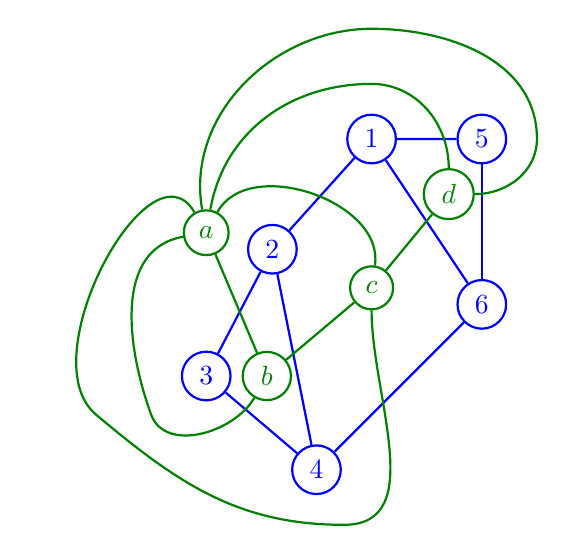
\begin{tikzpicture}[main/.style = {draw, circle, thick, color = Blue}, scale=0.7]
		\node[main] (4) at (0,0) {4};
		\node[main] (3) at (-2,1.7) {3};
		\node[main] (6) at (3,3) {6};
		\node[main] (2) at (-0.8,4) {2};
		\node[main] (5) at (3,6) {5};
		\node[main] (1) at (1,6) {1};
		\node[main, color=Green] (b) at (-0.9, 1.7) {$b$};
		\node[main, color=Green] (a) at (-2, 4.3) {$a$};
		\node[main, color=Green] (c) at (1, 3.3) {$c$};
		\node[main, color=Green] (d) at (2.4, 5) {$d$};
		\draw[thick, color=Blue] (4) edge (3);
		\draw[thick, color=Blue] (4) edge (2);
		\draw[thick, color=Blue] (4) edge (6);
		\draw[thick, color=Blue] (5) edge (6);
		\draw[thick, color=Blue] (6) edge (1);
		\draw[thick, color=Blue] (2) edge (1);
		\draw[thick, color=Blue] (1) edge (5);
		\draw[thick, color=Blue] (2) edge (3);
		\draw[thick, color=Green] (b) edge (c);
		\draw[thick, color=Green] (d) edge (c);
		\draw[thick, color=Green] (b) edge (a);
		
		\coordinate (6') at (4,2);
		\coordinate (3') at (-3, 1);
		
		\draw[thick, color=Green] (b) to[out = 240, in = -70] (3') to[out = 110, in = 190] (a);
		\draw[thick, color=Green, bend left = 80] (a) edge (c);
		\draw[thick, color=Green] (c) to[out=270,in=0] (.5,-1) to[out=180,in=-40] (-4,1) to[out=140, in=120] (a); %TODO
		\draw[thick, color=Green] (d) to[out=90,in=0] (1,7) to[out=180,in=80] (a);
		\draw[thick, color=Green] (d) to[out=0,in=270] (4,6) to[out=90,in=0] (1,8) to[out=180, in=100] (a);
	\end{tikzpicture}
	\caption{A \textcolor{Blue}{primal graph $G$} and its \textcolor{Green}{dual $\dual{G}$}.}
\end{figure}

Also duals in Matroids (and also minors) were inspired from graphs. Now we have encountered only planar graphs. But one can ask what about non-planar ones. By Kuratowsku and the fact that graphic matroids are closed under minor operations we get the following proposition.

\begin{prop}
	$\dual{\M}(K_5)$ (and $\dual{\M}(K_{3,3})$) are not graphic.
\end{prop}

\begin{proof}
	By a contradiction: $\exists G : \M(G) = \dual{G}(K_5)$. By that $|E| = 10, \rank(\dual{\M}(K_5)) = 6 = 10 -4$. Also $|V(G)| = 7$ so average degree is $\frac{20}{7} < 3$. Which means that there exists a vertex $v$ s.t. $\deg(v) = 1$ or 2. This leads to at most 2 edges therefore the size of min edge cut is 2 and so is the size of co-circuit of $\dual{\M}(K_5)$ hence the size of circuit in $\M(K_5)$ is 2 which is a contradiction. Similar argument can be made for $K_{3,3}$.
\end{proof}

From these facts if we have a non-planar graph its dual is \textbf{not graphic}. Therefore we get the following diagram.

\begin{figure}[!ht]\centering
	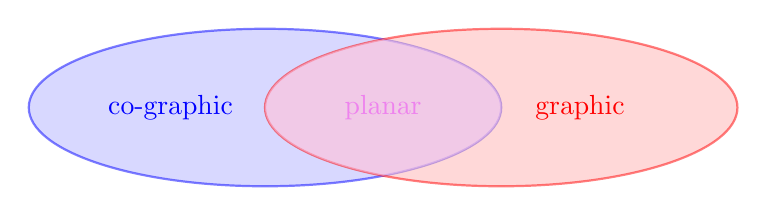
\begin{tikzpicture}[thick]
		\draw[Blue, fill=Blue!30, opacity=.5] (0,0) ellipse (3cm and 1cm);
		\node[Blue] at (-1.2,0) {co-graphic};
		\draw[Red, fill=Red!30, opacity=.5] (3,0) ellipse (3cm and 1cm);
		\node[Red] at (4,0) {graphic};
		\begin{scope}
			\clip (0,0) ellipse (3cm and 1cm);
			\clip (3,0) ellipse (3cm and 1cm);
			\fill[Violet, fill=Violet!40, opacity=.5] (2,0) ellipse (2cm and 1cm);
		\end{scope}
		\node[Violet] at (1.5,0) {planar};
	\end{tikzpicture}
	\caption{Diagram of graphic duals.}
\end{figure}

	\chapter{Algorithms}
\end{document}
